\documentclass[conference]{IEEEtran}
\usepackage[T1]{fontenc}
\usepackage[utf8]{inputenc}
\usepackage{amsmath,amssymb,graphicx,booktabs,array}
\usepackage[hidelinks]{hyperref}
\usepackage{url}
\newcommand{\code}[1]{\texttt{#1}}
\title{Evidence-Grounded Clinical Trial Screening with a Compact Transformer: Adaptation and Explicit Inference Mechanisms}
\author{\IEEEauthorblockN{Muhammad Harris Azhar}
\IEEEauthorblockA{National University of Computer and Emerging Sciences\\Student ID: i232535\\Generative AI --- Assignment 2}}
\begin{document}
\maketitle
\begin{abstract}
Clinical trial screening requires interpreting individual eligibility criteria while distinguishing negative evidence from missing information. This work adapts the open-weight Qwen3-4B-Instruct-2507 model to produce criterion-level categories and original patient-sentence citations. The prescribed TrialGPT annotations are partitioned by patient, with 37 training, eight validation and eight held-out test patients. Completion-only quantized low-rank adaptation uses 602 usable training records. Validation accuracy increases from 0.3738 to 0.7524. On all 206 held-out records, accuracy increases from 0.4078 to 0.7427, macro-F1 from 0.3492 to 0.4733, and evidence micro-F1 from 0.4571 to 0.5714, while rare negative categories remain difficult. Explicit cache-aware decoding obtains validated speedups of 1.42--4.17 times on matching workloads; one long-output cached/uncached mismatch remains documented. A tiled online-softmax implementation agrees numerically with a controlled reference and reduces peak allocated memory by approximately 51.5\% at length 512, but is slower than dense attention. Greedy speculative decoding with Qwen3-0.6B passes all six correctness cases and 54 timed trials, with workload-dependent speed ratios of 0.652--1.361. A browser application exposes exact evidence, preliminary aggregation, live decoding comparisons and report export. The results distinguish improved aggregate scores from remaining category and evidence failures.
\end{abstract}
\begin{IEEEkeywords}
clinical trial eligibility, evidence retrieval, QLoRA, KV cache, online softmax, speculative decoding
\end{IEEEkeywords}

\section{Introduction}
Matching a patient's narrative history to a clinical trial involves more than identifying a disease keyword. Inclusion requirements may depend on numerical thresholds, chronology and treatment history; exclusion conditions may depend on explicit negation or comorbidities. A missing laboratory result does not establish either that a threshold is met or that it is violated. A useful research prototype must preserve these distinctions and connect predictions to the actual patient record.

The assignment addresses criterion-level screening rather than independently labeled trial-level enrollment. The system accepts a numbered patient description, the criterion type and criterion text, and predicts an applicable expert category plus supporting sentence IDs. It retains insufficient-information and not-applicable categories. The application aggregates individual judgments through explicit rules; that aggregate is not presented as a ground-truth patient--trial outcome.

The implementation investigates whether a small open-weight decoder can be adapted on freely available compute, and how inference mechanisms behave under controlled measurements. Contributions are: (1) leakage-aware preparation and completion-only adaptation; (2) strict category/citation evaluation and traceable explanations; (3) explicit cache-aware and uncached greedy paths; (4) dense and tiled online-softmax attention; (5) manual greedy speculative decoding; and (6) a standalone browser workflow with live comparisons and export. The implementation uses original experiment outputs and reports failures rather than assuming every optimization is faster.

\section{Related Work and Design Alternatives}
TrialGPT decomposes patient-to-trial matching into retrieval, criterion-level matching and ranking, including evidence localization and explanations~\cite{trialgpt}. This project adopts the criterion-level problem and public annotations, but implements its own adaptation, evaluation, attention, decoding and application. It does not run the original repository as the submitted system. The annotations contain previous model outputs, which are excluded from all input features.

LoRA freezes base weights and learns low-rank updates~\cite{lora}. QLoRA combines low-rank adaptation with a quantized frozen model, reducing adaptation memory~\cite{qlora}. These approaches are suitable for a small supervised dataset and a free T4 runtime, but neither guarantees clinical reasoning quality or eliminates activations, temporary allocations and optimizer memory. Full fine-tuning was rejected as unnecessarily demanding for the available hardware and limited data.

The Qwen3 family provides open decoder models at several sizes~\cite{qwenreport}. The selected July instruction checkpoint is a direct-response, non-thinking model~\cite{qwen4}. A 3B alternative reduces weights but has unmeasured task-specific quality; a 7B alternative increases memory. Table~\ref{tab:models} records plausible alternatives, not an empirical leaderboard. Estimated 16-bit storage is parameter count times two bytes and excludes runtime overhead.

\begin{table}[t]\centering\small
\caption{Model alternatives considered. GB estimates concern weights only.}\label{tab:models}
\resizebox{\columnwidth}{!}{\begin{tabular}{lrrl}\toprule
Model & Parameters & 16-bit GB & License\\\midrule
Qwen2.5-3B-Instruct & 3.09B & 6.2 & Qwen Research\\
Qwen3-4B-Instruct-2507 & 4.0B & 8.0 & Apache 2.0\\
Qwen2.5-7B-Instruct & 7.61B & 15.2 & Apache 2.0\\\bottomrule
\end{tabular}}
\end{table}
Official model cards establish candidate specifications~\cite{qwen3candidate,qwen7candidate}. Qwen3-4B was selected for its capacity/resource compromise, updated instruction post-training, permissive license and accessible causal forward interface. Parameter count alone is not evidence of superior clinical reasoning. Cross-model clinical accuracy was not measured; the controlled classification comparison uses the same target before and after adaptation.

FlashAttention motivates tiling and online normalization to reduce attention's memory traffic~\cite{flash}. The educational implementation here uses ordinary PyTorch operations and does not claim a fused kernel or the paper's hardware efficiency. Speculative decoding uses a cheap draft and parallel target verification~\cite{specpaper}. This work implements deterministic greedy prefix matching, rather than the paper's probabilistic rejection-sampling algorithm. Assisted-generation APIs are not the submitted algorithm, and published acceleration claims are not transferred to the measured pair.

\section{Materials and Methods}
\subsection{Dataset Integrity and Fixed Patient Split}
The mandatory TrialGPT Criterion Annotations dataset~\cite{dataset} contains 1,015 annotations over 53 patients. Each row includes a patient description, criterion type/text, expert category and expert evidence sentences, along with metadata and prior model outputs. Only the three permitted clinical input fields enter prompts. Annotation, patient and trial identifiers are preserved as metadata, while expert labels/evidence are separate targets.

Unique patient IDs are sorted and shuffled by NumPy \code{default\_rng(42)}. The first 37 form training, the next eight validation, and the last eight testing. All annotations for a patient remain in one group. The published manifest records IDs and annotation counts: 603 raw training, 206 validation and 206 test annotations. Training annotation 883 has missing criterion text and is explicitly quarantined, leaving 602 usable training examples; it is not silently counted as a training record. Invalid validation/test records are not silently removed. No prompt, model, threshold or checkpoint is selected with test labels.

Original numbered patient lines are parsed with consecutive IDs starting at zero. Sentence splitting is not repeated, preserving annotation alignment. Input and target schemas, missingness, label sets, duplicates, patient overlap and lengths are checked. Preparation records model/tokenizer revisions, hashes, versions and a zero-truncation policy.

\subsection{Target Architecture and Structured Interface}
The target checkpoint has approximately four billion parameters, 36 decoder layers, hidden size 2,560, 32 query heads and eight key/value heads, head dimension 128, RoPE positional encoding and model vocabulary size 151,936~\cite{qwen4}. Its native context capability is 262,144 tokens; the project's frozen budget is 1,024 tokens with 128 reserved for generation. Development prompts fit without truncation; the selected budget is a project constraint rather than the model's native limit.

\begin{figure*}[t]\centering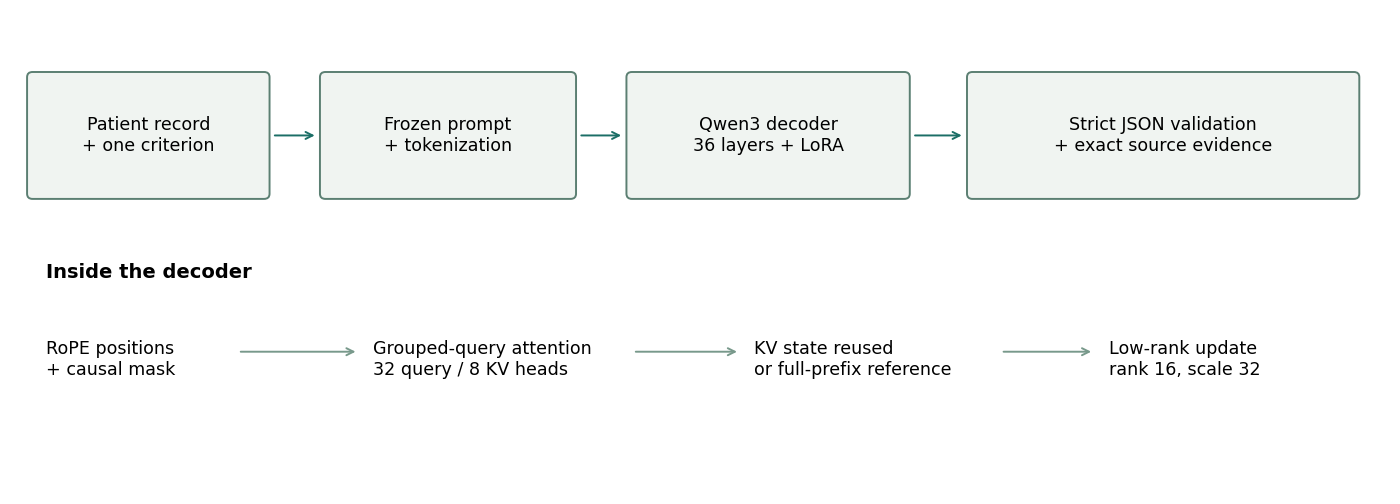
\includegraphics[width=.94\textwidth]{generated/architecture.png}\caption{System architecture and target decoder components. The browser supplies permitted inputs; model decisions are validated before original record statements are retrieved. Cache state and low-rank adaptation have distinct roles.}\label{fig:architecture}\end{figure*}
Figure~\ref{fig:architecture} places model adaptation, cache handling and evidence extraction within the complete workflow. The educational tiled-attention implementation is assessed separately rather than silently replacing target attention.

The prompt explicitly describes applicable inclusion and exclusion labels, negation, thresholds, chronology, missing information and citation rules. The output is exactly two JSON keys: \code{label} and \code{sentence\_ids}. Inclusion categories are included, not included, not enough information and not applicable. Exclusion categories are excluded, not excluded, not enough information and not applicable. The strict parser rejects markdown wrappers, extra keys, duplicate/negative/noninteger IDs, invalid category assignments and nonexistent citations. Invalid responses remain in evaluation denominators and are not repaired.

\subsection{Adaptation Objective and Checkpoint Selection}
The base is loaded in 4-bit NF4 with double quantization and FP16 computation. LoRA targets linear modules with rank 16, scale 32 and dropout 0.05. Adam-style optimization uses learning rate $10^{-4}$, weight decay 0.01, gradient norm limit 1.0, warmup ratio 0.1, batch size one and accumulation over eight examples. Gradient checkpointing limits activation memory. Three epochs produce 228 optimizer steps. There are 33,030,144 trainable parameters, approximately 0.8145\% of the reported total after adapter injection.

Only expert completion tokens receive the autoregressive cross-entropy loss:
\begin{equation}
\mathcal L=-\frac{1}{|C|}\sum_{t\in C}\log p_\theta(y_t\mid x,y_{<t}),
\end{equation}
where $C$ excludes prompt and padding positions. Tests verify masking, prefix alignment, nonempty targets, no overlength truncation and exclusion of validation patients from training. Checkpoint 76, at the end of epoch one, is selected by lowest validation completion loss, not classification F1. Training takes 2,707.25 seconds on a T4, with 6.03 GiB peak allocated and 9.73 GiB peak reserved memory.

\begin{figure*}[t]\centering
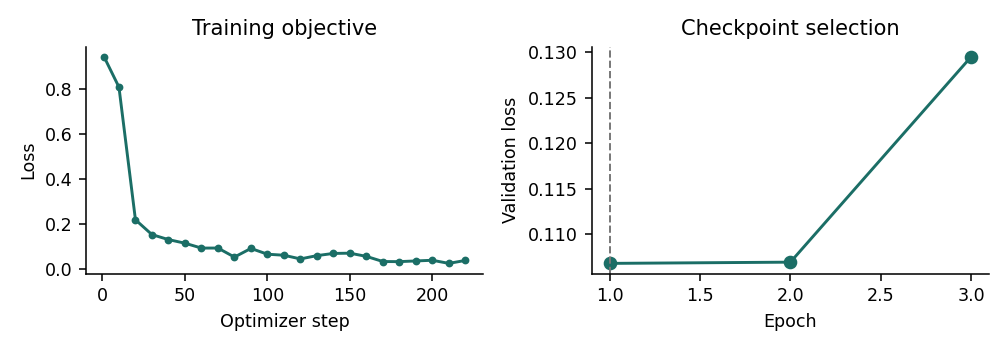
\includegraphics[width=.91\textwidth]{generated/training_curve.png}
\caption{Recorded training objective and validation completion loss. Validation loss is approximately 0.106814, 0.106949 and 0.129507 across epochs; the selected adapter comes from epoch one despite completion of all three epochs.}\label{fig:training}
\end{figure*}

\subsection{Eligibility, Evidence and Explanations}
The prediction parser evaluates structure, label validity and citation validity separately. Exact supporting text is recovered by original sentence ID. Explanations are deterministic descriptions of the category and quoted evidence, not a second unsupported generative reasoning chain. When evidence is absent or a response invalid, the interface exposes the gap rather than inventing a rationale.

The preliminary application aggregate follows ordered rules: invalid or unsupported decisions require review; explicit negative inclusion/exclusion labels identify a potential conflict; insufficient information requests additional information; all-not-applicable inputs produce no applicable assessment; otherwise applicable criteria are provisionally satisfied. A prediction of included or not excluded without any citation is flagged for review. These are screening rules, not independently evaluated enrollment labels.

\subsection{Explicit KV-Cached and Uncached Generation}
Both paths use model forwards and deterministic argmax selection. The uncached reference reprocesses the growing prefix on every step. The cached path prefills the prompt once, then supplies the new token with past key/value tensors. Attention masks cover past plus current positions; RoPE positions use the absolute sequence index. Caches are fresh for each request and are inspected for token growth and tensor byte count. With prompt length $P$ and $N$ emitted tokens, the final cache contains $P+N-1$ processed tokens because the last emitted token has not yet been forwarded.

Correctness compares manual cached, manual uncached and HF reference outputs. CUDA synchronization brackets timing. Prefill, decode, total latency, actual output throughput and allocator peaks are recorded with warmup and three repetitions; min/max and raw trials are retained. Controlled stress tests fix output work by disabling EOS; complete clinical prompts retain normal EOS behavior. Cache tensors add memory, so acceleration is not described as a universal memory reduction.

\subsection{Dense and Tiled Online-Softmax Attention}
The dense reference computes scaled scores $S=QK^\top/\sqrt d$, applies the causal mask where requested, subtracts row maxima and normalizes before multiplying by $V$. The tiled variant processes key/value blocks and maintains running row maximum $m$, normalizer $\ell$ and unnormalized output $A$. For a new block with scores $S_b$:
\begin{align}
m'&=\max(m,\max_j S_{b,j}),\\
\ell'&=e^{m-m'}\ell+\sum_j e^{S_{b,j}-m'},\\
A'&=e^{m-m'}A+e^{S_b-m'}V_b.
\end{align}
The final output is $A/\ell$ where $\ell>0$, and zero for fully masked rows. Causal offsets, grouped-query heads and finite values are checked. Low-precision inputs accumulate in FP32; the controlled experiment uses FP32 tensors. The implementation never calls SDPA inside the tiled path. Separate reference, tiled and automatic SDPA measurements distinguish conceptual tiling from an optimized backend.

\subsection{Manual Greedy Speculative Decoding}
The draft is the smaller pinned Qwen3-0.6B model~\cite{qwendraft}. Actual configured fast-tokenizer backends, vocabulary mappings and special IDs are compared before loading weights. Both tokenizers expose 151,669 configured entries and the models share 151,936 output rows. EOS is 151645, pad is 151643 and BOS is absent. Raw merges files differ, so they are independently hash-checked rather than asserted byte-identical. Only the target chat template formats inputs; its exact token IDs are supplied to the draft.

Each decoder owns separate target/draft caches. A normal round starts with caches covering committed tokens except the last. The draft proposes at most $K$ candidates, respecting EOS and remaining budget. One target forward on the pending committed suffix plus the candidate block yields $K+1$ next-token distributions. Only the consecutive candidate prefix matching target argmax tokens is accepted. On rejection, the target correction is emitted; on complete acceptance and remaining budget, a target bonus is emitted. Rejected suffixes are cropped, and the draft cache is synchronized when a bonus leaves it behind. Every round emits at least one token and neither stale candidates nor excess-budget tokens survive.

The controlled GPU study uses NF4 target weights with FP32 computation and math SDPA, and FP16 draft computation. It is separate from the original FP16 classification/KV runs. This precision control follows earlier near-tie sensitivity; it does not make finite-precision equality a theorem. All six preflight cases compare ordinary greedy against HF and speculative against ordinary before timing. Mismatches remain failures, with diagnostics preserved and no silent fallback. Both models remain resident in all timed modes, including ordinary greedy.

\section{Experimental Setup and Metrics}
Recorded GPU experiments use a Tesla T4, CUDA 13.0, torch 2.14.1+cu130, Transformers 5.15.1, PEFT 0.21.2, bitsandbytes 0.50.2 and accelerate 1.15.0. Model, tokenizer, adapter, input and source hashes are recorded. Before/after classification uses the same validation examples, frozen prompt, 4-bit weights, FP16 computation and greedy decoding. The application's CUDA protocol instead uses FP32 computation; CPU deployment uses unquantized FP32. Classification scores from another precision are not automatically attributed to those deployment paths.

Classification metrics are accuracy, fixed-label macro-F1, per-class precision/recall/F1 and confusion matrices, overall and separately by criterion type. Zero-support applicable classes stay in the macro average; invalid predictions remain errors. Evidence scores operate on citation sets: $TP=|G\cap P|$, $FP=|P\setminus G|$, $FN=|G\setminus P|$. Precision, recall and F1 use these counts. Both sets empty yields one; one set empty yields zero. Micro scores pool counts and macro scores average examples; nonempty-gold-only macro scores are also saved to expose the influence of empty evidence.

The KV grid has prompt lengths 128/256/512 crossed with budgets 16/32/64 and three repetitions per mode, totaling 54 timings. Three full clinical prompts are separate correctness checks. Attention uses lengths 128/256/512, full and causal masks, shape $[1,4,L,64]$, and five repetitions per method: 90 timings. Speculation uses stress pairs 128/16, 256/32 and 512/64 plus three full clinical prompts, two draft lengths and ordinary greedy, with three repetitions: 54 timings. Loading, tokenization, plotting and warmup are outside generation timing. Speculative drafting, verification, comparisons, synchronization and rollback are inside it.

\section{Results and Discussion}
\subsection{Validation Before and After Adaptation}
\begin{table*}[t]\centering\small\caption{Development validation comparison. Evidence F1 is pooled sentence-retrieval micro-F1; valid denotes strict output validity.}\label{tab:validation}\begin{tabular}{llrrrrr}
\toprule
Group & Model & N & Accuracy & Macro F1 & Evidence F1 & Valid \\
\midrule
overall & Original & 206 & 0.3738 & 0.2924 & 0.5258 & 0.9903 \\
overall & Adapted & 206 & 0.7524 & 0.4438 & 0.6154 & 1.0000 \\
inclusion & Original & 66 & 0.6818 & 0.4115 & 0.6446 & 1.0000 \\
inclusion & Adapted & 66 & 0.7424 & 0.3857 & 0.7288 & 1.0000 \\
exclusion & Original & 140 & 0.2286 & 0.1693 & 0.3288 & 0.9857 \\
exclusion & Adapted & 140 & 0.7571 & 0.4192 & 0.4062 & 1.0000 \\
\bottomrule
\end{tabular}
\end{table*}
Table~\ref{tab:validation} and Fig.~\ref{fig:validation} show a 37.86 percentage-point accuracy improvement. Correct responses increase from 77 to 155 of 206. All adapted outputs are valid, versus 204 original outputs. Evidence micro-F1 increases by 0.0896. Most category improvement arises in exclusion criteria: accuracy increases from 0.2286 to 0.7571. This is not evidence that every class or subgroup improved.

\begin{figure}[t]\centering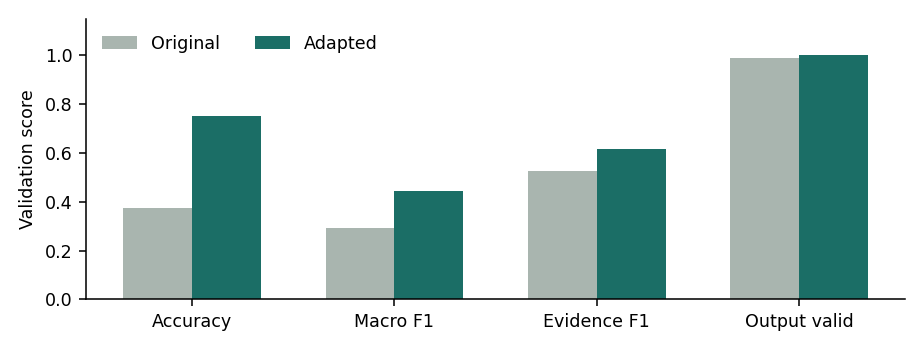
\includegraphics[width=\columnwidth]{generated/validation_comparison.png}\caption{Overall validation comparison under the frozen FP16 classification protocol. Accuracy gains exceed macro-F1 gains, indicating unequal improvement across categories.}\label{fig:validation}\end{figure}

\begin{table}[t]\centering\small\caption{Adapted model: per-class validation performance.}\label{tab:classes}\begin{tabular}{lrrrr}
\toprule
Category & N & Precision & Recall & F1 \\
\midrule
included & 35 & 0.897 & 0.743 & 0.812 \\
not included & 3 & 0.000 & 0.000 & 0.000 \\
excluded & 2 & 0.000 & 0.000 & 0.000 \\
not excluded & 101 & 0.772 & 0.941 & 0.848 \\
not enough information & 53 & 0.620 & 0.585 & 0.602 \\
not applicable & 12 & 1.000 & 0.250 & 0.400 \\
\bottomrule
\end{tabular}
\end{table}
Table~\ref{tab:classes} exposes the main limitation: all three not-included cases and both excluded cases are missed. Inclusion accuracy rises, but its macro-F1 decreases from 0.4115 to 0.3857. The inclusion not-included class loses its one original correct response, while some larger categories improve. The sparse negative supports make class-specific conclusions unstable. Overall evidence precision is 0.8358 and recall 0.4870; the model retrieves 56 gold citations and misses 59. High precision therefore coexists with incomplete evidence retrieval, particularly for exclusion criteria.

\begin{figure}[t]\centering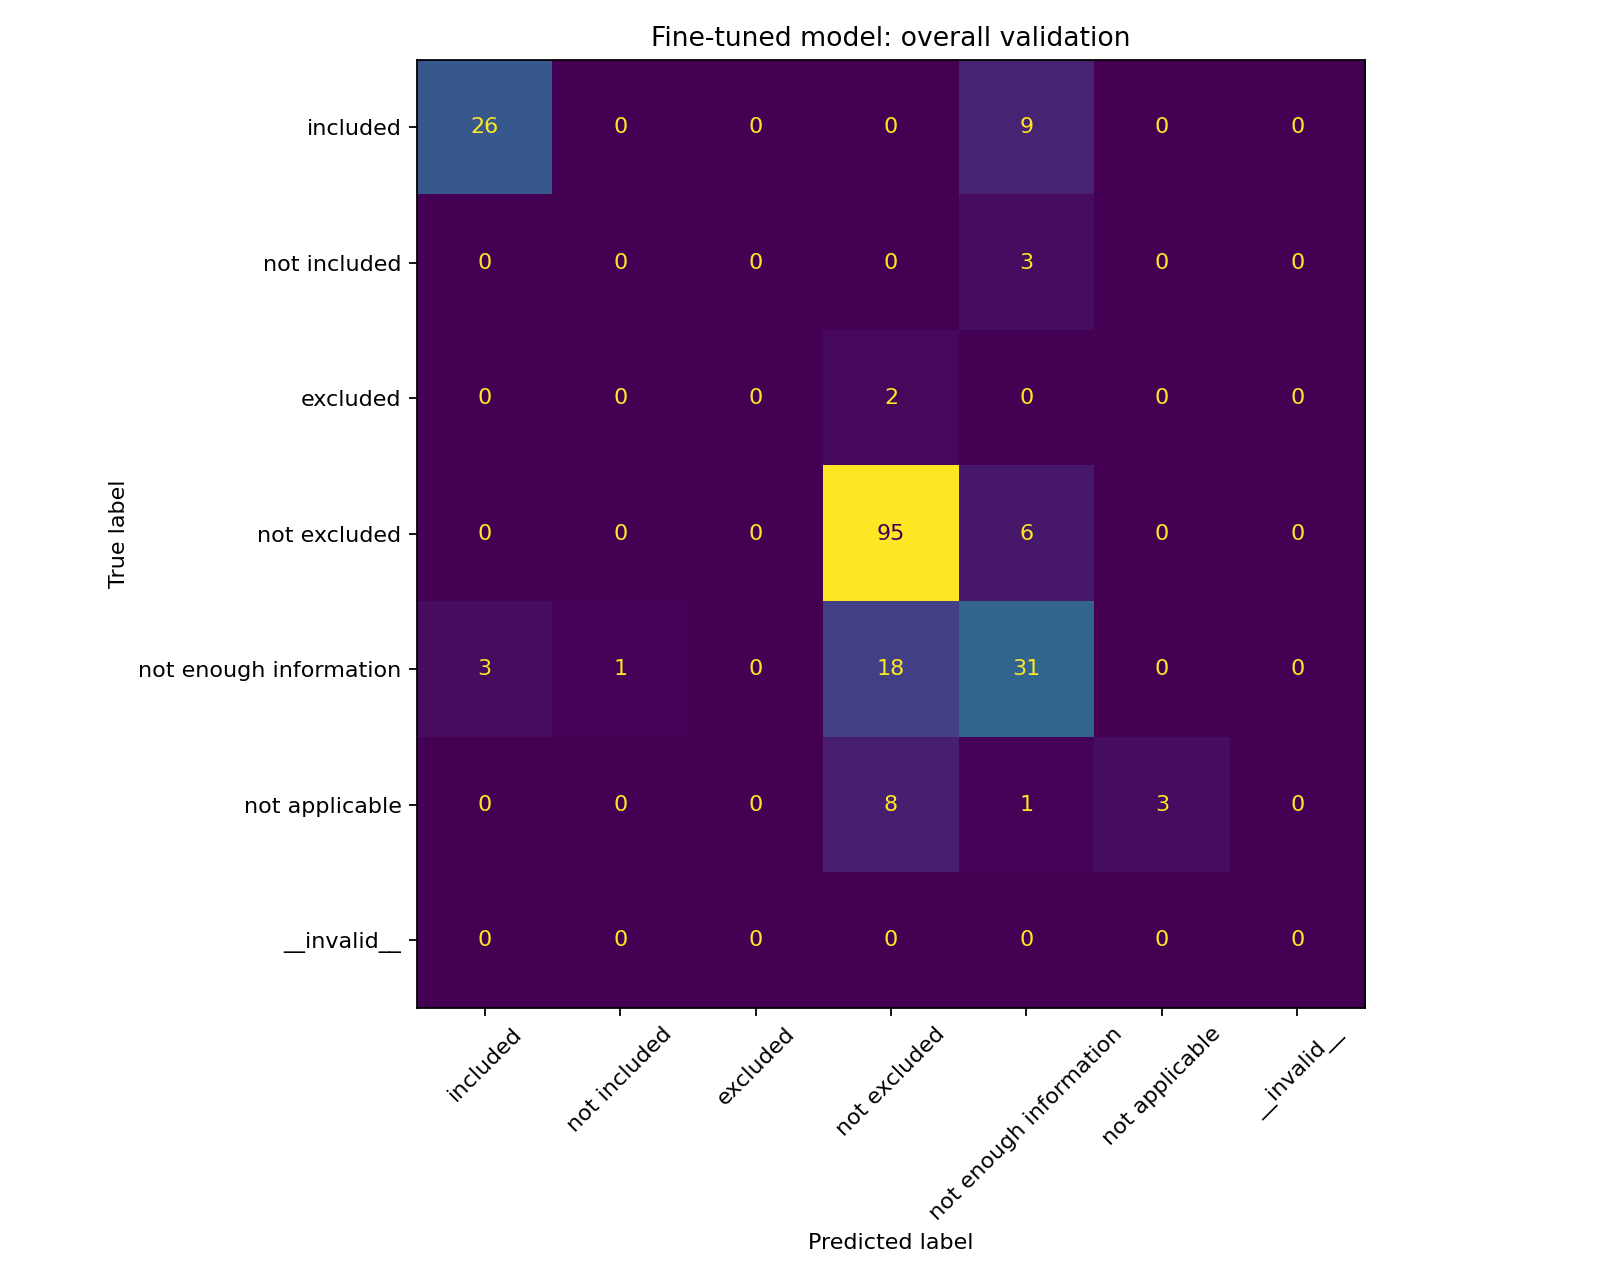
\includegraphics[width=\columnwidth]{../results/finetuning_qlora_v1/validation/confusion_overall.png}\caption{Adapted-model validation confusion matrix, retaining the invalid-prediction category. Rare negative classes and confusion between missing information and not excluded remain visible.}\label{fig:confusion}\end{figure}
The confusion matrix in Fig.~\ref{fig:confusion} supports the interpretation that learning the frequent not-excluded category drives much of the accuracy gain. The model never predicts excluded in this validation run. Eighteen of 26 exclusion examples with gold insufficient-information labels are predicted not excluded. Such errors are consequential because missing documentation must not become evidence that an exclusion condition is absent.

\subsection{Final Held-Out Evaluation Status}
The final held-out comparison is complete. Table~\ref{tab:test} reports all 206 annotations from the reserved eight patients. Original and adapted phases use the same frozen base, quantization, prompt, greedy decoding and automatic SDPA; the adapter is disabled only for the original phase. The returned predictions were independently checked against the original source inputs and expert targets, re-parsed with the frozen strict parser, and all classification/evidence metrics were recomputed. No subsequent tuning is performed.
\begin{table*}[t]\centering\small\caption{Final held-out test results, separate from development validation.}\label{tab:test}\begin{tabular}{llrrrr}
\toprule
Group & Model & N & Accuracy & Macro F1 & Evidence F1 \\
\midrule
overall & before & 206 & 0.4078 & 0.3492 & 0.4571 \\
inclusion & before & 75 & 0.7067 & 0.5815 & 0.5524 \\
exclusion & before & 131 & 0.2366 & 0.1905 & 0.1714 \\
overall & after & 206 & 0.7427 & 0.4733 & 0.5714 \\
inclusion & after & 75 & 0.7600 & 0.5802 & 0.6847 \\
exclusion & after & 131 & 0.7328 & 0.3508 & 0.2222 \\
\bottomrule
\end{tabular}
\end{table*}
Accuracy improves from 0.4078 (84/206) to 0.7427 (153/206), a gain of 33.50 percentage points. Overall macro-F1 rises from 0.3492 to 0.4733. Inclusion accuracy increases from 0.7067 to 0.7600, but inclusion macro-F1 falls slightly from 0.5815 to 0.5802. Exclusion accuracy rises from 0.2366 to 0.7328 and macro-F1 from 0.1905 to 0.3508. Both phases produce valid JSON/categories/citations for every test record; validity is not the same as clinical correctness.

Table~\ref{tab:testclasses} preserves every applicable category and zero-support class. The not-excluded category improves from 2/91 to 89/91 correct, explaining much of the aggregate gain. Not-included recall falls from 3/7 to 1/7, while not-applicable recall falls from 11/15 to 3/15. Included recall is unchanged at 20/27. These regressions prevent describing adaptation as uniformly better. There are no gold excluded examples in this test group, so excluded sensitivity cannot be estimated; its zero score remains in the fixed applicable macro-F1 rather than silently removing the class.
\begin{table*}[t]\centering\footnotesize\caption{Final test category metrics overall and by criterion type. P/R/F1 denotes precision/recall/F1; zero-support classes remain.}\label{tab:testclasses}\begin{tabular}{lrrr}
\toprule
Group / category & N & Before P/R/F1 & After P/R/F1 \\
\midrule
overall / included & 27 & 0.909/0.741/0.816 & 0.909/0.741/0.816 \\
overall / not included & 7 & 0.300/0.429/0.353 & 0.333/0.143/0.200 \\
overall / excluded & 0 & 0.000/0.000/0.000 & 0.000/0.000/0.000 \\
overall / not excluded & 91 & 1.000/0.022/0.043 & 0.736/0.978/0.840 \\
overall / not enough information & 66 & 0.369/0.727/0.490 & 0.702/0.606/0.650 \\
overall / not applicable & 15 & 0.268/0.733/0.393 & 1.000/0.200/0.333 \\
inclusion / included & 27 & 0.909/0.741/0.816 & 0.909/0.741/0.816 \\
inclusion / not included & 7 & 0.300/0.429/0.353 & 0.333/0.143/0.200 \\
inclusion / not enough information & 38 & 0.778/0.737/0.757 & 0.714/0.921/0.805 \\
inclusion / not applicable & 3 & 0.286/0.667/0.400 & 1.000/0.333/0.500 \\
exclusion / excluded & 0 & 0.000/0.000/0.000 & 0.000/0.000/0.000 \\
exclusion / not excluded & 91 & 1.000/0.022/0.043 & 0.736/0.978/0.840 \\
exclusion / not enough information & 28 & 0.213/0.714/0.328 & 0.625/0.179/0.278 \\
exclusion / not applicable & 12 & 0.265/0.750/0.391 & 1.000/0.167/0.286 \\
\bottomrule
\end{tabular}
\end{table*}
Evidence micro-F1 improves from 0.4571 to 0.5714. Adapted micro precision is 0.7925 and recall 0.4468 (42 true positives, 11 false positives and 52 false negatives). Table~\ref{tab:testevidence} includes micro/macro precision, recall and F1, with nonempty-gold-only F1. Of 206 records, 145 have empty gold evidence; consequently macro-F1 of 0.8343 substantially exceeds the nonempty-only value of 0.5553. Exclusion evidence recall is only 0.1250, so improved label accuracy must not obscure weak support retrieval.
\begin{table*}[t]\centering\scriptsize\caption{Final held-out evidence metrics with the explicit empty-set policy. Nonempty F1 is example-macro F1 restricted to nonempty gold.}\label{tab:testevidence}\begin{tabular}{llrrrrrrr}
\toprule
Group & Model & Micro P & Micro R & Micro F1 & Macro P & Macro R & Macro F1 & Nonempty F1 \\
\midrule
overall & before & 0.6957 & 0.3404 & 0.4571 & 0.8191 & 0.8131 & 0.8127 & 0.4165 \\
overall & after & 0.7925 & 0.4468 & 0.5714 & 0.8455 & 0.8328 & 0.8343 & 0.5553 \\
inclusion & before & 0.6744 & 0.4677 & 0.5524 & 0.6764 & 0.6700 & 0.6668 & 0.5113 \\
inclusion & after & 0.7755 & 0.6129 & 0.6847 & 0.7356 & 0.7109 & 0.7130 & 0.6771 \\
exclusion & before & 1.0000 & 0.0938 & 0.1714 & 0.9008 & 0.8950 & 0.8962 & 0.1500 \\
exclusion & after & 1.0000 & 0.1250 & 0.2222 & 0.9084 & 0.9027 & 0.9038 & 0.2125 \\
\bottomrule
\end{tabular}
\end{table*}
\begin{figure}[t]\centering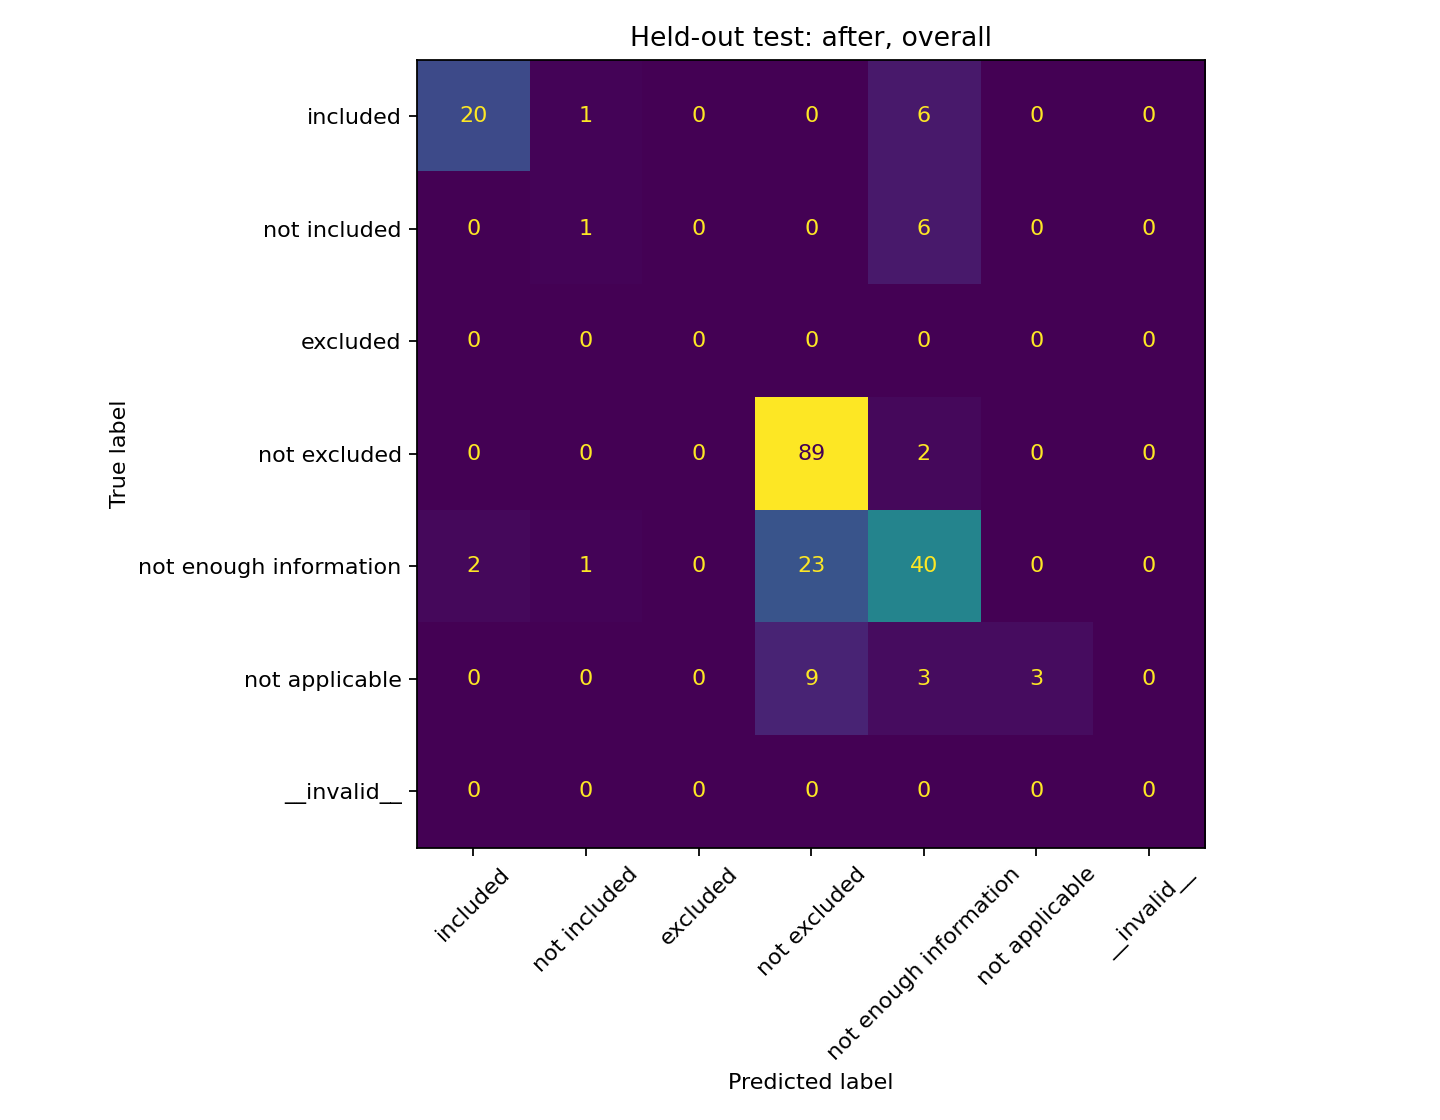
\includegraphics[width=\columnwidth]{../results/final_test/confusion_after_overall.png}\caption{Selected model's final held-out confusion matrix. Sparse/absent categories and remaining missing-information errors constrain interpretation.}\label{fig:testconfusion}\end{figure}
Figure~\ref{fig:testconfusion} visualizes these remaining errors. The eight examples in the later error-analysis section are drawn from these completed held-out predictions, after every model and prompt choice was fixed; they are analyzed for reporting, not fed back into training.


\subsection{KV Cache: Speedup and a Remaining Disagreement}
\begin{table}[t]\centering\small\caption{KV-cache math-SDPA study. Ratios are uncached/cached median total latency; unequal output suppresses validated speedup.}\label{tab:kv}\begin{tabular}{lrrr}
\toprule
Input/output case & Cached (s) & Uncached (s) & Speedup \\
\midrule
p128-o16 & 2.291 & 3.249 & 1.42 \\
p128-o32 & 4.962 & 7.180 & 1.45 \\
p128-o64 & 9.268 & 15.955 & 1.72 \\
p256-o16 & 2.421 & 5.883 & 2.43 \\
p256-o32 & 4.710 & 12.483 & 2.65 \\
p256-o64 & 9.746 & 24.402 & 2.50 \\
p512-o16 & 2.848 & 9.912 & 3.48 \\
p512-o32 & 4.978 & 20.775 & 4.17 \\
p512-o64 & 10.066 & 42.639 & unequal \\
\bottomrule
\end{tabular}
\end{table}
All 54 timed calls finish. Eight of nine stress cases and all three full clinical cases pass token equality; cached manual generation agrees with HF in all 12 correctness cases. For matching stress workloads, Table~\ref{tab:kv} shows 1.42--4.17 times acceleration. Longer prompts increase the cost of repeatedly recomputing the full prefix, while cache reuse processes one new token after prefill.

The automatic-SDPA experiment first disagreed at output index five for length 256. At the same prefix, uncached top-two logits differed by 0.015625, while cached logits tied; maximum absolute logit difference was 0.0390625. A focused math-SDPA control resolved that case. The full math study still disagrees at index 43 for the 512/64 stress case. That residual numerical disagreement was not repaired, dropped or declared passing. The user closed further investigation, so the report preserves the overall failed correctness flag. Timing completion is distinct from correctness completion.

Allocated peaks are approximately 2.699--2.814 GiB cached and 2.684--2.773 GiB uncached. These include resident weights and temporary tensors, not only KV storage. Raw artifacts retain prefill/decode breakdown, throughput, allocator peaks and cache bytes. This study does not establish unconditional bit-identical decoding across computation shapes or an across-the-board memory benefit.

\subsection{Attention: Numerical Agreement and a Memory/Latency Trade-Off}
\begin{table*}[t]\centering\small\caption{Standalone FP32 attention on T4. Peaks are measured allocated MiB including inputs and intermediates; SDPA auto does not identify a particular fused kernel.}\label{tab:attention}\begin{tabular}{lrrrrr}
\toprule
Length / mask & Dense ms & Tiled ms & SDPA ms & Dense MiB & Tiled MiB \\
\midrule
128 / full & 0.876 & 2.709 & 0.292 & 9.26 & 9.00 \\
128 / causal & 1.045 & 2.583 & 0.299 & 9.26 & 9.00 \\
256 / full & 1.406 & 7.888 & 0.324 & 11.89 & 9.50 \\
256 / causal & 1.329 & 6.719 & 0.330 & 11.89 & 9.50 \\
512 / full & 1.415 & 28.808 & 0.673 & 21.66 & 10.50 \\
512 / causal & 1.584 & 22.205 & 0.677 & 21.66 & 10.50 \\
\bottomrule
\end{tabular}
\end{table*}
All six shapes/masks pass the configured numerical checks. Maximum tiled absolute error is $6.9123\times10^{-7}$. Table~\ref{tab:attention} and Fig.~\ref{fig:attention} show that at length 512 the measured peak falls from 21.656 to 10.505 MiB, approximately 51.5\% lower. A 64-by-64 FP32 score tile occupies 64 KiB compared with the dense 4 MiB score matrix, but that theoretical 64-times score-workspace ratio is not the measured total-memory ratio.

\begin{figure*}[t]\centering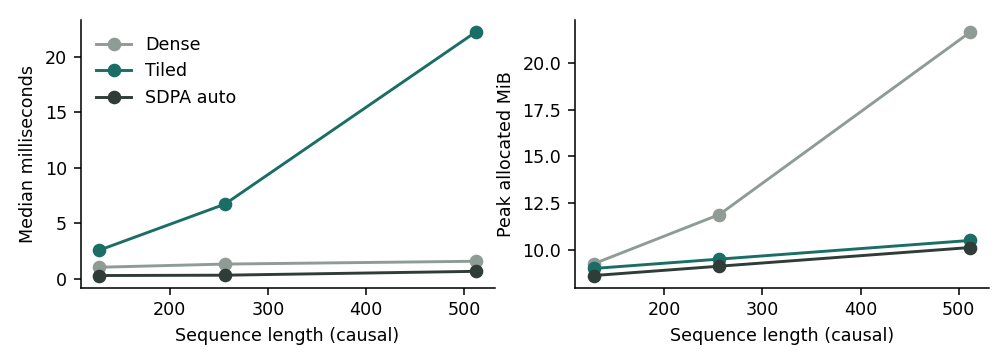
\includegraphics[width=.9\textwidth]{generated/attention_tradeoff.png}\caption{Causal attention runtime and allocator peaks. Educational Python tiling saves memory at larger lengths while running slower; automatic SDPA is fastest in these measurements.}\label{fig:attention}\end{figure*}
The tiled path is slower in every GPU case; automatic SDPA is fastest. Python loops, repeated small operations, kernel launches and allocations can overwhelm the saved memory traffic. A fused IO-aware kernel performs scheduling that this implementation does not reproduce. These are standalone tensor experiments; the custom attention module is not inserted into Qwen, and no end-to-end clinical-model acceleration is claimed. CPU checks also pass, with unavailable native GPU-memory fields represented as null rather than invented measurements.

\subsection{Speculation: Correct Outputs with Mixed Speed Outcomes}
All six preflight cases and all 54 timings pass exact equality against ordinary target greedy. Table~\ref{tab:spec} summarizes acceptance and speed ratios; Fig.~\ref{fig:spec} shows actual median latency.
\begin{table*}[t]\centering\small\caption{Speculative GPU comparison. Speed is ordinary greedy/speculative median latency; values below one are slowdowns. Both models remain resident.}\label{tab:spec}\begin{tabular}{lrrrrr}
\toprule
Case & Greedy (s) & K2 speed & K2 accept \% & K4 speed & K4 accept \% \\
\midrule
p128-o16 & 2.871 & 1.316 & 83.3 & 1.361 & 81.2 \\
p256-o32 & 4.814 & 0.870 & 34.2 & 0.652 & 27.0 \\
p512-o64 & 9.675 & 1.075 & 76.5 & 0.950 & 56.2 \\
clinical-938 & 3.496 & 0.861 & 36.8 & 0.789 & 31.0 \\
clinical-6 & 3.361 & 1.093 & 61.5 & 0.967 & 42.9 \\
clinical-243 & 3.898 & 0.907 & 36.8 & 0.817 & 31.0 \\
\bottomrule
\end{tabular}
\end{table*}
\begin{figure*}[t]\centering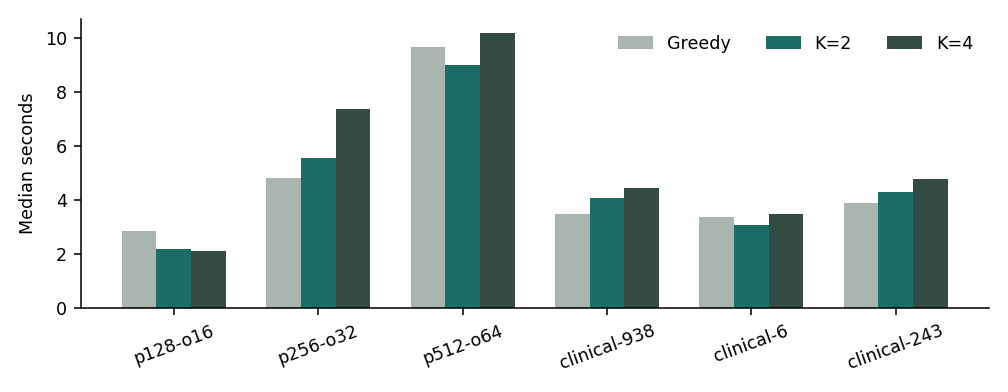
\includegraphics[width=.91\textwidth]{generated/speculative_latency.png}\caption{Measured ordinary and speculative latency on identical prompts with a shared FP32 target protocol. Draft length four is slower on most cases despite fewer target forwards.}\label{fig:spec}\end{figure*}
K=2 is faster in three of six workloads; K=4 is faster only on the shortest stress workload. Ratios span 0.652--1.361. In the 256/32 case, K=4 reduces target forwards from 32 to 16 but requires 64 draft forwards and accepts only 27.0\% of proposals, so total latency increases. On the shortest stress case it reduces target forwards to four and attains the best ratio. Reducing expensive forwards is therefore insufficient by itself: acceptance, draft cost, proposal length, host logic and synchronization jointly determine latency.

Clinical outputs are short, limiting amortization. K=2 acceptance varies from approximately 36.8\% to 61.5\% across the three clinical prompts, with two clinical slowdowns and one modest gain. These six development prompts do not estimate a production latency distribution. Memory includes both models in ordinary and speculative modes; the experiment does not measure a standalone target-only deployment comparison. The earlier FP16 KV times are not used as speculative baselines because target precision differs.

\section{Representative Error Analysis}
The following eight distinct adapted-model held-out records are selected from completed final predictions after every model and prompt choice was fixed. Expert annotations are the evaluation reference, not independent clinical adjudications performed in this project. Full raw outputs, note text and exact gold/predicted citations are supplied in \code{reports/final\_test\_error\_cases.json}; earlier development cases remain separately preserved.
\paragraph{1. Negative inclusion failure (annotation 162)}
Criterion (inclusion): Patients undergoing open abdominal aortic aneurysm repair Expert: not included; model: not enough information. Gold IDs []; predicted IDs [0]. The category conflicts with the reference; a citation does not by itself justify the interpretation.

\paragraph{2. Negative inclusion failure (annotation 163)}
Criterion (inclusion): Patients undergoing endovascular abdominal aneurysm repair Expert: not included; model: not enough information. Gold IDs []; predicted IDs [0]. The category conflicts with the reference; a citation does not by itself justify the interpretation.

\paragraph{3. Negative inclusion failure (annotation 164)}
Criterion (inclusion): Patients undergoing surgical lower limb revascularisation (suprainguinal or infrainguinal) Expert: not included; model: not enough information. Gold IDs []; predicted IDs [0]. The category conflicts with the reference; a citation does not by itself justify the interpretation.

\paragraph{4. Missing information resolved without support (annotation 174)}
Criterion (exclusion): Patients with previous axillary surgery Expert: not enough information; model: not excluded. Gold IDs []; predicted IDs []. The category conflicts with the reference; a citation does not by itself justify the interpretation.

\paragraph{5. Missing information resolved without support (annotation 193)}
Criterion (exclusion): Patients were moribund. Expert: not enough information; model: not excluded. Gold IDs [0, 1, 2, 3, 4]; predicted IDs []. The category conflicts with the reference; a citation does not by itself justify the interpretation.

\paragraph{6. Not-applicable criterion misinterpreted (annotation 165)}
Criterion (exclusion): Pregnancy Expert: not applicable; model: not excluded. Gold IDs []; predicted IDs []. The category conflicts with the reference; a citation does not by itself justify the interpretation.

\paragraph{7. Not-applicable criterion misinterpreted (annotation 422)}
Criterion (inclusion): If female, using birth control Expert: not applicable; model: not enough information. Gold IDs [3]; predicted IDs [3]. The category conflicts with the reference; a citation does not by itself justify the interpretation.

\paragraph{8. Incomplete evidence despite matching category (annotation 179)}
Criterion (exclusion): Had been performed central venous puncture or catheterization before. Expert: not excluded; model: not excluded. Gold IDs [0]; predicted IDs []. The category agrees but the source evidence set is incomplete or differs from the reference.

The negative-inclusion and not-applicable groups illustrate contradictory interpretations relative to the annotated reference. Missing-information cases expose unsupported resolution of unknowns. Evidence discrepancies show that a plausible category does not imply complete support localization. These observations motivate manual review and future research, but no follow-up tuning is performed on the final test group. Explanations quote the record and distinguish model judgment from verified clinical fact.

\section{Integrated Browser Application}
TrialScreen provides one browser workspace with a patient record editor, separately entered inclusion/exclusion criteria, per-criterion categories, exact evidence text and clickable source sentence IDs. Unnumbered lines are numbered deterministically; already numbered records preserve their IDs. Invalid numbering, empty criteria, excessive request sizes and over-context prompts return actionable errors rather than silent truncation. All criterion budgets are checked before producing decisions.

The application exposes live cached/uncached and optional speculative comparisons on the first entered criterion. Comparisons share a target, inputs, precision and math SDPA, record three repetitions after warmup, retain raw token IDs, and suppress validated speedups for mismatches. CPU peaks unavailable to the CUDA allocator are shown as missing, not zero. Both loaded models remain resident when comparing speculation. This is an executable comparison rather than a screenshot-only benchmark panel.

Screening reports export as readable HTML or JSON with note text, criteria, predictions, exact quotes, preliminary aggregation rules, model revision, adapter hashes, precision and timestamp. Text is escaped in HTML. The loopback server accepts only local origins, serves an explicit static-file allowlist, limits JSON request size, and runs one model operation at a time. Patient input is held in memory and not automatically written to disk. This local research server is not an internet-facing clinical service.

\begin{figure*}[t]\centering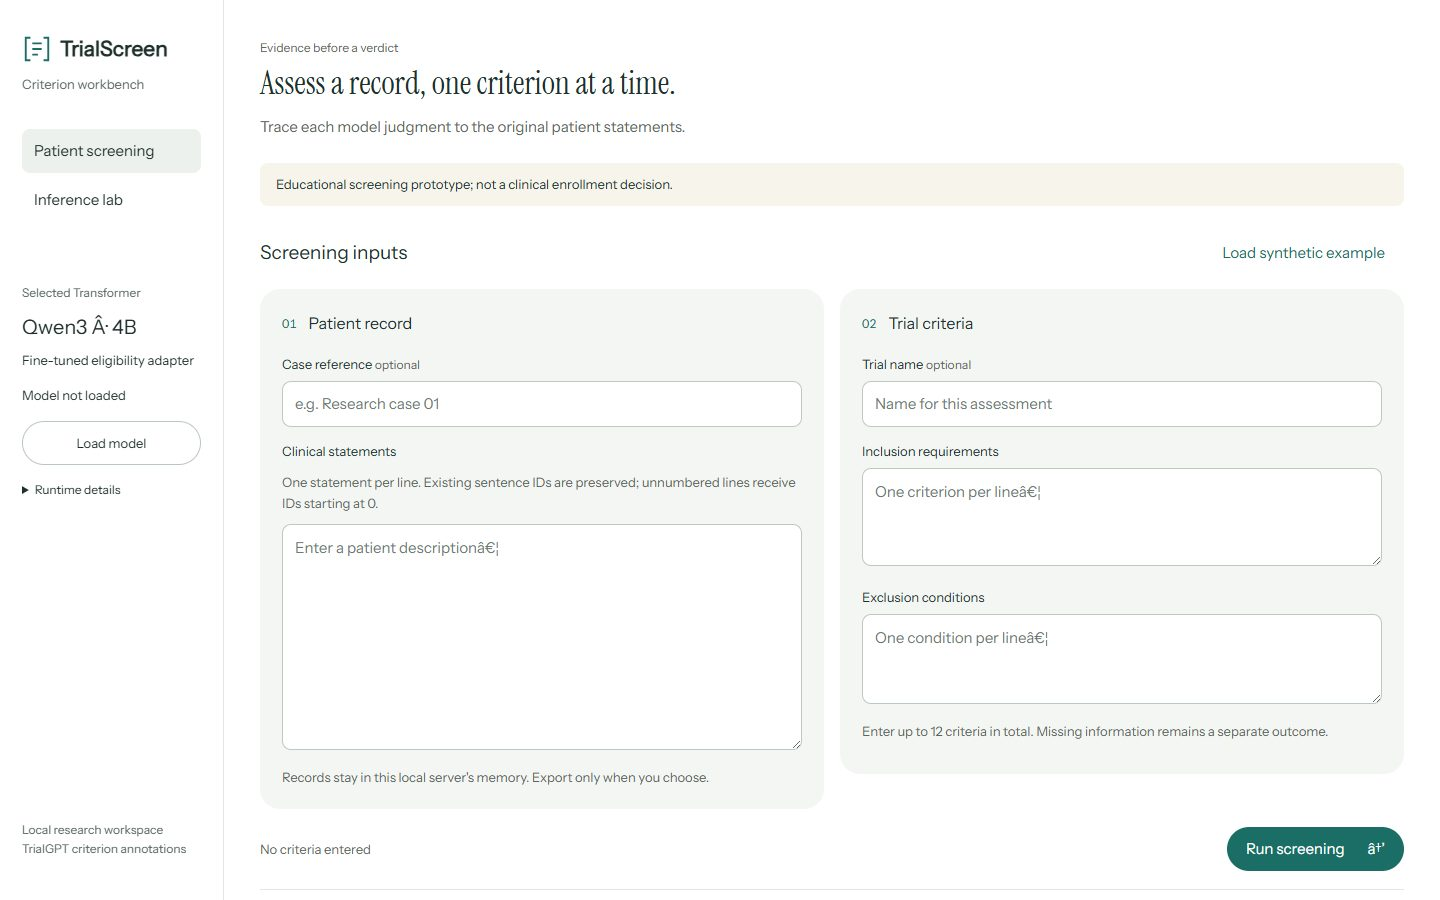
\includegraphics[width=.92\textwidth]{generated/application.jpg}\caption{Actual browser input workspace. The screenshot illustrates the interface state, not a new clinical inference result. Desktop/mobile layout, invalid-input recovery, sample filling and navigation were checked with a real headless browser.}\label{fig:app}\end{figure*}
Figure~\ref{fig:app} shows the standalone interface. Windows startup is provided through a double-click launcher; an evaluator uses browser controls once the host is started. Setup and resource requirements are documented. Full-size model inference on this CPU-only laptop has not been independently benchmarked; actual CUDA model experiments occurred in Colab. The service's forward integration is tested with real miniature Qwen3 models, and API/export behavior is tested separately. Those checks are not misrepresented as full-size end-to-end deployment validation.

\section{Limitations and Reproducibility}
The dataset is small and heavily imbalanced; a patient-level split reduces leakage but leaves very few rare negatives for development estimates. Synthetic descriptions and annotation policy may differ from longitudinal clinical records. Category accuracy and citation correctness do not establish clinical safety, and the model's supporting text may not logically justify its category. Fixed context rejection preserves evidence but limits arbitrary long-note usage. The program does not retrieve live trial registries or decide enrollment.

The residual KV mismatch remains unresolved. Precision/backend changes can influence near-tie argmax decisions, so deterministic greedy configuration alone does not imply identical finite-precision outputs across shapes. Speculative equality is verified for the tested cases, not every possible prompt. Tiled attention is an educational module with measured slowdowns, not a fused replacement for the target's attention. The application's FP32 deployment protocol and CPU resource demand differ from the classification experiment.

Reproduction artifacts include the source dataset checksum, fixed split, tokenizer locks, model revisions, completion masking tests, selected adapter hashes, training history, raw predictions, benchmark repetitions, scripts, notebooks and environment specifications. Source/data bundling preserves exact bytes; a Windows CRLF-to-LF notebook-export bug was reproduced and corrected without disabling checksum validation. Reruns reject changed identities and preserve failed preflight evidence. The final checklist records the required repository, adapter and video publication links rather than inventing inaccessible URLs.

\section{Conclusion}
A four-billion-parameter open decoder can be adapted on free T4 resources for structured criterion-level screening with traceable sentence citations. Held-out accuracy reaches 74.27\% and evidence micro-F1 0.5714, but rare negative categories, not-applicable judgments and evidence recall remain weaknesses. Cache reuse improves matching-workload latency while exposing a numerical corner case; explicit online-softmax tiling trades runtime for memory; and speculative decoding is correct on the measured suite with both gains and slowdowns. The result is a research screening prototype with transparent limitations, not an enrollment decision system. Development evidence, held-out assessment and deployment verification remain separate claims.

\appendices
\section{AI-Use Statement}
An OpenAI Codex coding assistant was used to help plan implementation, write and review code, debug environment and numerical issues, assemble experiment analyses, and draft this report. Existing PyTorch, Transformers, PEFT, bitsandbytes, NumPy, pandas and matplotlib libraries are acknowledged. The original TrialGPT project and scholarly sources informed design but were not substituted for the submitted implementation. Automated tests and artifact checks are supplied; the student remains responsible for validating outputs, understanding each component and defending or modifying it during evaluation. No AI-generated unmeasured scores are presented as experiment results.

\section{Source Project and Recorded Demonstration}
The submitted implementation, reproducibility instructions and report source project are hosted at:\\
\url{https://github.com/Harris-05/transformer-implementation}.
The recorded application demonstration supplied by the author is available at:\\
\url{https://youtu.be/-zL3ECuJL1A}.
The submission archive also includes the actual selected adapter and its training/validation artifacts in \code{finetuning\_results.zip}. Base and draft weights are obtained by their pinned model identifiers. Repository files should match the final source archive accompanying this paper.

\begin{thebibliography}{12}
\bibitem{trialgpt} Q. Jin \emph{et al.}, ``Matching patients to clinical trials with large language models,'' \emph{Nature Communications}, vol. 15, article 9074, 2024, doi: \href{https://doi.org/10.1038/s41467-024-53081-z}{10.1038/s41467-024-53081-z}.
\bibitem{lora} E. J. Hu \emph{et al.}, ``LoRA: Low-rank adaptation of large language models,'' arXiv:2106.09685, 2021. \url{https://arxiv.org/abs/2106.09685}.
\bibitem{qlora} T. Dettmers, A. Pagnoni, A. Holtzman, and L. Zettlemoyer, ``QLoRA: Efficient finetuning of quantized LLMs,'' arXiv:2305.14314, 2023. \url{https://arxiv.org/abs/2305.14314}.
\bibitem{qwenreport} A. Yang \emph{et al.}, ``Qwen3 technical report,'' arXiv:2505.09388, 2025. \url{https://arxiv.org/abs/2505.09388}.
\bibitem{qwen4} Qwen Team, ``Qwen3-4B-Instruct-2507,'' model card and pinned configuration, 2025. \url{https://huggingface.co/Qwen/Qwen3-4B-Instruct-2507}.
\bibitem{qwen3candidate} Qwen Team, ``Qwen2.5-3B-Instruct,'' official model card. \url{https://huggingface.co/Qwen/Qwen2.5-3B-Instruct}.
\bibitem{qwen7candidate} Qwen Team, ``Qwen2.5-7B-Instruct,'' official model card. \url{https://huggingface.co/Qwen/Qwen2.5-7B-Instruct}.
\bibitem{flash} T. Dao, D. Y. Fu, S. Ermon, A. Rudra, and C. R\'e, ``FlashAttention: Fast and memory-efficient exact attention with IO-awareness,'' arXiv:2205.14135, 2022. \url{https://arxiv.org/abs/2205.14135}.
\bibitem{specpaper} Y. Leviathan, M. Kalman, and Y. Matias, ``Fast inference from Transformers via speculative decoding,'' arXiv:2211.17192, 2023. \url{https://arxiv.org/abs/2211.17192}.
\bibitem{dataset} NCBI, ``TrialGPT Criterion Annotations,'' public-domain dataset. \url{https://huggingface.co/datasets/ncbi/TrialGPT-Criterion-Annotations}.
\bibitem{qwendraft} Qwen Team, ``Qwen3-0.6B,'' model card, Apache-2.0. \url{https://huggingface.co/Qwen/Qwen3-0.6B}.
\end{thebibliography}
\end{document}
